\documentclass{article}
\usepackage{verbatim}
\usepackage{amsmath}
\usepackage[margin=1in,left=1.5in,includefoot]{geometry}
\usepackage{graphicx}
\usepackage{systeme}
\usepackage{listings}
\usepackage{color}
\usepackage{xcolor}
\usepackage{graphicx}
\usepackage{biblatex}
\usepackage{float}
\usepackage{hyperref}
\usepackage{placeins}
\usepackage{fancyhdr}
\definecolor{mygreen}{RGB}{28,172,0} % color values Red, Green, Blue
\definecolor{mylilas}{RGB}{170,55,241}
\pagestyle{fancy}
\fancyhead{}
\fancyfoot{}
\fancyfoot[R]{ \thepage\ }
\usepackage[utf8]{inputenc}

% Default fixed font does not support bold face
\DeclareFixedFont{\ttb}{T1}{txtt}{bx}{n}{12} % for bold
\DeclareFixedFont{\ttm}{T1}{txtt}{m}{n}{12}  % for normal

% Custom colors
\usepackage{color}
\definecolor{deepblue}{rgb}{0,0,0.5}
\definecolor{deepred}{rgb}{0.6,0,0}
\definecolor{deepgreen}{rgb}{0,0.5,0}

\addbibresource{Reference3.bib}
\begin{document}


\begin{titlepage}
  \begin{center}
  \huge{Yujin Liu, Helen Jin, Jiangmeng Li}
  \end{center}


\end{titlepage}


\section{Introduction to the SIR Model and Notation}
The susceptible-infected-removed (SIR) model is one of the compartmental models that simplify the mathematical modeling to the spread of infectious disease, where the time dependent variables $S$, $I$, $R$ each represent the following populations:

$S$(susceptible): number of individuals who are not infected but could become infected

$I$(infected): number of individuals who are already infected and can spread disease

$R$(removed): number of individuals who are either recovered and immune or have died

And $s$, $i$, $r$ are used to represent the proportion of susceptible, infected and removed individuals among the population.

There are two parameters $b$ and $k$ in the model, where $b$ indicates the number of contacts each day by an individual who can spread the disease and $k$ indicates the fraction of the infectious population which recovers each day.

In the ODE-based model, we can get the following system of differential equations, where $t$ is time:

$\frac{ds}{dt} = -b * s(t) * i(t)$

$\frac{dr}{dt} = k * i(t)$

$\frac{di}{dt} = b * s(t) * i(t) - k * i(t)$
\section{Python Package 'sir'}


\section{Results of Simulations}
\subsection{Discrete Agent-Based Model}

To investigate how a new disease spreads, we run the simulations with both discrete agent-based model and continuous ODE model, starting with 100 infectious individuals among a total population of 20000.

We generate several plots to show how s, i, and r change during the simulation for different choices of k and b. First we check the plots for b = 2, which means we assume each individual has two interactions each day that could spread the disease, with different k values.

\begin{figure}[htp]

\centering
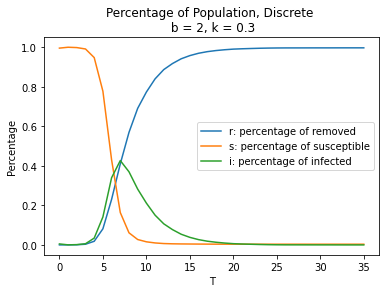
\includegraphics[width=.3\textwidth]{Figure1_discrete_sir_b2_k1.png}\hfill
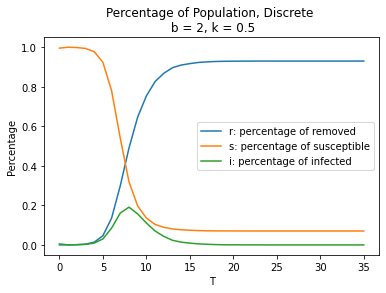
\includegraphics[width=.3\textwidth]{Figure1_discrete_sir_b2_k2.png}\hfill
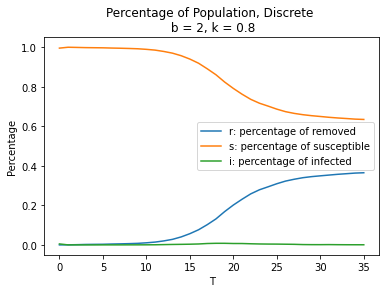
\includegraphics[width=.3\textwidth]{Figure1_discrete_sir_b2_k3.png}

\caption{Percentage of population susceptible (s), infected (i), and removed (r), discrete}
\label{fig:figure3}

\end{figure}



From the plots, we find that when the recovery rate is low (0.3), finally all people are removed, which indicates that all people were infectious and either have recovered and are now immune, or have died. As the recovery rate rises to a high level (0.8), the trends change obviously. The percentage of infected people does not increase, and the percentage of removed people increases to approximately 0.4 while the percentage of susceptible people decreases to 0.6. Finally, both trends of removed and susceptible people stays constant. In this case, there are fairly large proportion of individuals who are never infected. Thus, when the recovery rate k is large enough (larger than 0.6) and b is relatively small (less than 3), then the herd immunity is eventually achieved. The herd immunity occurs when a large portion of a community becomes immune to a disease, making the spread of disease unlikely, so the whole community becomes protected. Next, we increase the value of b and see whether the trends change.


\begin{figure}[htp]

\centering
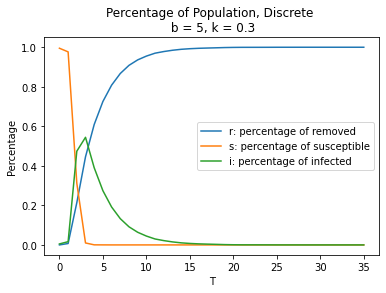
\includegraphics[width=.3\textwidth]{Figure1_discrete_sir_b5_k1.png}\hfill
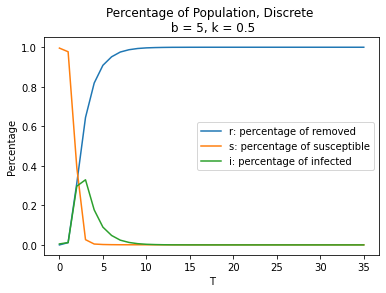
\includegraphics[width=.3\textwidth]{Figure1_discrete_sir_b5_k2.png}\hfill
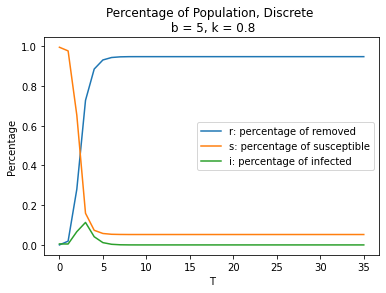
\includegraphics[width=.3\textwidth]{Figure1_discrete_sir_b5_k3.png}

\caption{Percentage of population susceptible (s), infected (i), and removed (r), discrete}
\label{fig:figure3}

\end{figure}



When b = 5, each individual has five interactions each day that could spread the disease. These plots suggest that when each individual get contacts with five infectious people per day, if the recovery rate is 0.3, then finally all people are removed after 20 days; if the recovery rate is 0.5, all people are removed after 10 days; even if the recovery rate is 0.8, less than 10$\%$ of individuals will remain susceptible after 10 days. As a result, when b is large enough, no matter how large k is, almost all people will be removed eventually, which means that all people will be infected and left with different results. Hence, people should avoid contacting in person with infectious people. Some suggestions include staying at home as much as possible and avoiding visiting areas where the disease is prevalent.


Now, we want to investigate some qualitative behaviors of the simulations based on the parameters b and k in the phase diagrams.
The simulations are done with T values 10, 20 and 30 days for both discrete and continuous cases.


\begin{figure}[htp]

\centering
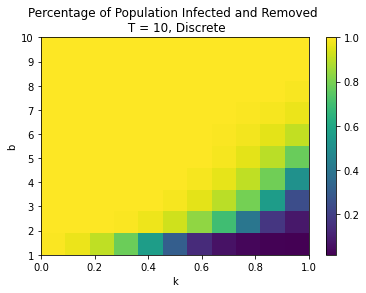
\includegraphics[width=.3\textwidth]{Figure1_discrete_diagT10total.png}\hfill
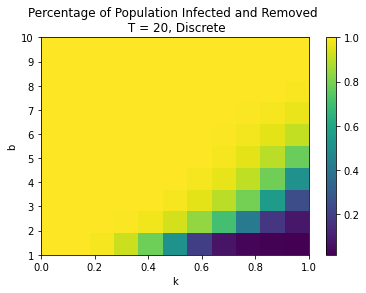
\includegraphics[width=.3\textwidth]{Figure1_discrete_diagT20total.png}\hfill
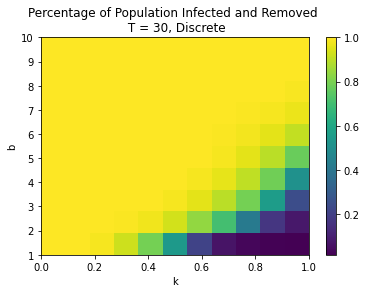
\includegraphics[width=.3\textwidth]{Figure1_discrete_diagT30total.png}

\caption{Phase diagrams for total percentage of population infected (i+r), discrete}
\label{fig:figure3}

\end{figure}



In figure 3, three phase diagrams illustrate the percentage of population infected and removed, i.e., the total percentage of population infected. It depends on both b, the number of interactions per day per individual that could spread the disease, and k, the recovery rate. The diagrams look very similar for different lengths of simulation (10, 20, and 30 days). It is clear that as k increases and b decreases, the total percentage of population infected decreases. If each individual only has less than two interactions per day that could spread the disease and the recovery rate is higher than 0.6, then almost nobody will be infected over time. The yellow area represents that everyone is eventually infected. When k is less or equal to 0.2, then everyone is eventually infected. Also, when b is larger than 6, everyone is eventually infected. Furthermore, when b is relatively small (less than 7) but k is relatively large (larger than 0.3), everyone is eventually infected. More precisely, the cut edge between the area where all individuals are infected and the remaining area is approximately linear, so that we may estimate the edge by $b = 10k - 3$. Therefore, when $b - 10k + 3 > 0$, everyone is eventually infected.

We set b is larger than 1 in the above simulations. However, b can be less than 1. For instance, b = 0.5 is equivalent to say, each individual has 50$\%$ chance to be infected by one interaction with infectious people per day.


\begin{figure}[htp]

\centering
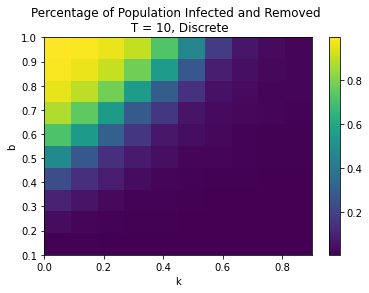
\includegraphics[width=.3\textwidth]{Figure1_discrete_bsmall_T10.png}\hfill
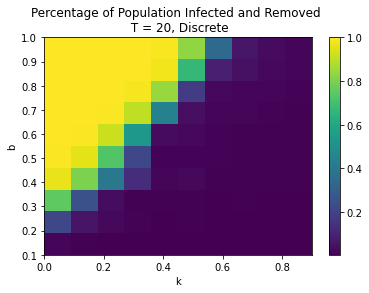
\includegraphics[width=.3\textwidth]{Figure1_discrete_bsmall_T20.png}\hfill
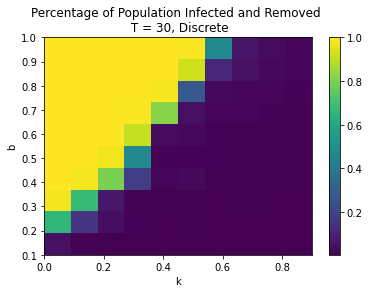
\includegraphics[width=.3\textwidth]{Figure1_discrete_bsmall_T30.png}

\caption{Phase diagrams for percentage of population infected and removed (i+r), discrete}
\label{fig:figure3}

\end{figure}


There are some interesting findings in figure 4. When T = 10, only when b is larger than 0.7 and k is smaller than 0.3, everyone is eventually infected. However, as T increases, the yellow area takes more space in the phase diagram, which means the range of parameters b and k is wider corresponding to where everyone is eventually infected. We do not observe effect of T in figure 3, but here it seems that for T = 30 even if b is really small and k is moderate, there still exists chance that everyone is infected.



\begin{figure}[htp]

\centering
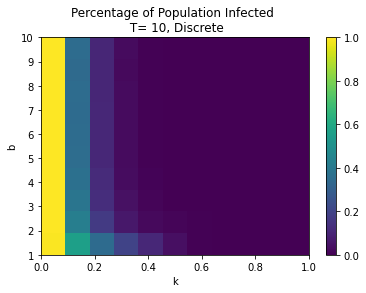
\includegraphics[width=.3\textwidth]{Figure1_discrete_diagT10infect.png}\hfill
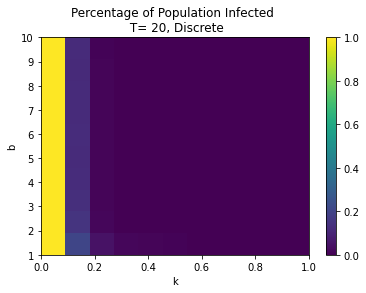
\includegraphics[width=.3\textwidth]{Figure1_discrete_diagT20infect.png}\hfill
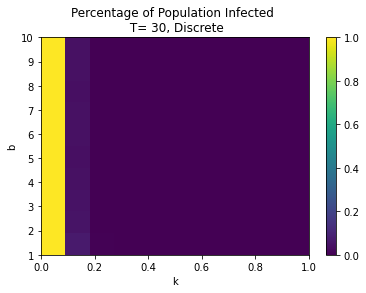
\includegraphics[width=.3\textwidth]{Figure1_discrete_diagT30infect.png}

\caption{Phase diagrams for percentage of population infected (i), discrete}
\label{fig:figure3}

\end{figure}


Then, we try to discover the parameter regimes that i will quickly go to 0. Figure 5 shows the phase diagrams for only infected population. We conclude that the percentage of infected people will quickly goes to 0, if the recovery rate k is large. Specifically, our simulations demonstrate when k is larger than 0.3, i will quickly go to 0 regardless of b.



\begin{figure}[htp]

\centering
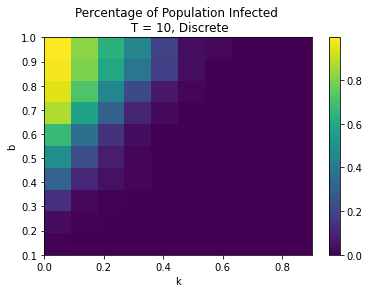
\includegraphics[width=.3\textwidth]{Figure1_discrete_bsmall_infectT10.png}\hfill
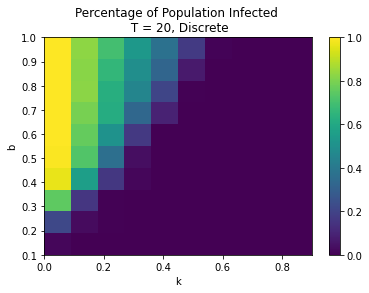
\includegraphics[width=.3\textwidth]{Figure1_discrete_bsmall_infectT20.png}\hfill
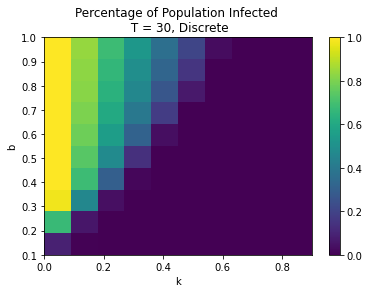
\includegraphics[width=.3\textwidth]{Figure1_discrete_bsmall_infectT30.png}

\caption{Phase diagrams for percentage of population infected (i), discrete}
\label{fig:figure3}

\end{figure}

Based on figure 6, when b is really small, the percentage of infected people can go to 0 even if the recovery rate k is small.




\subsection{Continuous/ODE-Based Model}











\section{Variations and Improvements}
\subsection{Modelling the usage of mask}
In this section, we study the effectiveness of mask in the spreading of the novel COVID-19 disease and develop a variation of the susceptible-infected-removed (SIR) model that provides a theoretical framework to investigate its spread within a community. More specifically, we will investigate how the use of mask will influence the percentage of deaths and hospitalizations with respect to different infectious contact rate.The model is based on the paper "To mask or not to mask: Modeling the potential for face mask use by the general public to curtail the COVID-19 pandemic" by Steffen E. Eikenberry et al. Although it is now recommended and a common practice to wear mask to limit the spread of COVID 19, it is very controversial at the beginning of the pandemic that whether it is neccesary and efficient to wear mask. So, we believe it is meaningful to understand quantitatively more about this topic.
In this model, we will introduce seven varaibles. S(t),E(t),I(t),H(t),A(t),R(t) each denote susceptible, exposed, symptomatic infectious, hospitalized, asymptomatic infectious, and recovered classes, with an assumption that people progress from \\
S $\rightarrow$ E $\rightarrow$ A $\rightarrow$ I $\rightarrow$H \\ At each state, infectious people will be able to recover, and only people in severe condition will go to hosptial and may die.\\D(t) is also included to track cumulative deaths. Two sets of ODE euqations will be used during simulation to find how use of mask will impact the spread of disease. We first consider a baseline model for the case where no masks are used. In the second set of ODEs, we will introduce more variables
$S_{U}(t)$,$E_{U}(t)$,$I_{U}(t)$,$H_{U}(t)$,$A_{U}(t)$,$R_{U}(t)$,$S_{M}(t)$,$E_{M}(t)$,$I_{M}(t)$,$H_{M}(t)$,$A_{M}(t)$,$R_{M}(t)$ to divide the population in two part: The population wearing masks and the one not wearing masks
Here are two sets of ODEs:\\
\begin{minipage}{0.45\textwidth}
\begin{eqnarray}
  \frac{dS}{dt} &=& -\beta{(t)}(I+\eta A)\frac{S}{N}\nonumber\\
  \frac{dE}{dt} &=& \beta(t)(I+\eta A)\frac{S}{N}-\sigma{E}\nonumber\\
  \frac{dI}{dt} &=& \alpha\sigma{E}-\phi{I}-\gamma_{I}I\nonumber\\
  \frac{dA}{dt} &=& (1-\alpha)\sigma E-\gamma_{A}A\nonumber\\
  \frac{dH}{dt} &=& \phi I - \sigma H - \gamma_{H}H\nonumber\\
  \frac{dR}{dt} &=& \gamma_{I}{I} + \gamma_{A}{A}+\gamma_{H}{H}\nonumber\\
  \frac{dD}{dt} &=& \sigma H\nonumber\\
\end{eqnarray}
\end{minipage}
\begin{minipage}{0.35\textwidth}
\tiny
\begin{eqnarray}
  \frac{dS_{U}}{dt} &=& -\beta(I_{U}+\eta A_{U})\frac{S_{U}}{N}-\beta((1-\epsilon_{0})I_{M}+(1-\epsilon_{0})\eta A_{M})\frac{S_{U}}{N}\nonumber\\
  \frac{dE_{U}}{dt} &=& \beta(I_{U}+\eta{A}_{U})\frac{S_{U}}{N}+\beta((1-\epsilon_{0})I_{M}+(1-\epsilon_{0})\eta A_{M}))\frac{S_{U}}{N}-\sigma E_{U}\nonumber\\
  \frac{dI_{U}}{dt} &=& \alpha\sigma E_{U}-\phi I_{U}-\gamma_{I}I_{U}\nonumber\\
  \frac{dA_{U}}{dt} &=& (1-\alpha)\sigma E_{U}-\gamma_{A}A_{U}\nonumber\\
  \frac{dH_{U}}{dt} &=& \phi I_{U}-\delta H_{U}-\gamma_{H}H_{U}\nonumber\\
  \frac{dR_{U}}{dt} &=& \gamma_{I}I_{U}+\gamma_{A}A_{U}+\gamma_{H}H_{U}\nonumber\\
  \frac{dD_{U}}{dt} &=& \delta H_{U}\nonumber\\
  \frac{dS_{M}}{dt} &=& -\beta(1-\epsilon_{i})(I_{U}+\eta A_{U})\frac{S_{M}}{N}-\beta(1-\epsilon_{i})((1-\epsilon_{0})I_{M}+(1-\epsilon_{0})\eta A_{M})\frac{S_{M}}{N}\nonumber\\
  \frac{dE_{M}}{dt} &=& \beta(1-\epsilon_{i})(I_{U}+\eta A_{U})\frac{S_{M}}{N}+\beta(1-\epsilon_{i})((1-\epsilon_{0})I_{M}+(1-\epsilon_{0})\eta A_{M})\frac{S_{M}}{N}-\sigma E_{M} \nonumber\\
  \frac{dI_{M}}{dt} &=& \alpha\sigma E_{M} - \phi I_{M}-\gamma_{I} I_{M}\nonumber\\
  \frac{dA_{M}}{dt} &=& (1-\alpha)\sigma E_{M}-\gamma_{A}A_{M}\nonumber\\
  \frac{dH_{M}}{dt} &=& \phi I_{M}-\delta H_{M}-\gamma_{H}H_{M}\nonumber\\
  \frac{dR_{M}}{dt} &=& \gamma_{I}I_{M} +\gamma_{A}A_{M}+\gamma_{H}H_{M}\nonumber\\
  \frac{dD_{M}}{dt} &=& \delta H_{M}\nonumber\\
\end{eqnarray}
\end{minipage}

We will run the simulation and observe what will happen in several days. \\Here,$\beta$ is the infectious contact rate, $\sigma$ is the transition exposed to infectious\\$\eta$ is the infectiousness factor for asymptomatic carriar, $\alpha$ is the fraction of infections that become symptomatic\\
$\phi$ is rate of hospitalization,$\gamma_{A}$ is the recovery rate for asymptomatic
\\$\gamma_{I}$ is the recovery rate, symptomatic,$\gamma_{H}$ is the recovery rate for hospitalized.\\$\sigma$ is the death rate in hospital.$\epsilon_{0}$ is the outward efficiency of the masks while $\epsilon_{i}$ is the inward efficiency of the masks.\\

We will find the default estimated values for all parameters with population masked and not masked.
Here, an assumption is made that the inward efficiency and outward efficiency of masks are the same($\epsilon_{0} = \epsilon_{1}$. We will draw a 2 dimensional phase diagram to show how the efficiency of mask(homemade mask or surgery mask) and the percentage of masked people will influence the hospitalization as well as the total deaths among the population.





\subsection{Fitting the data with SIR model}
In this section we will try to fit the SIR model with the SARS coronavirus. The SARS dataset in China will be collected from the link:\cite{SARSsource}

The dataset described the disease spread in China from 2003-03-17 to 2003-06-01, during which an emergency specialty field hospital was built on April 22nd in Beijing to treat the most severely infected individuals. Since the establishment of the hospital, the SARS coronavirus got controlled. In this model, we will try to simulate parameters and explore how the hospital as a major fator limited the spread of coronavirus. We will adopt the ODE simulation in the original SIR model to fit the data from 2003-03-17 to 2003-04-22 with choice of b and k. Then we introduce a new variable $\gamma_{H}$ to the model and come up with the following ODEs:
\begin{eqnarray}
  \frac{dS}{dt} &=& -\beta I*\frac{S}{N}*(1-\gamma_{H})\\
  \frac{dI}{dt} &=& \beta *\frac{S}{N}*I*(1-\gamma_{H})- k*I\\
  \frac{dR}{dt} &=& k*I\\
  \frac{dD}{dt} &=& \gamma_{H}*I*\delta\\
\end{eqnarray}

We will use data from 2003-03-17 to 2003-04-22 to find appropriate values of $\beta$, k as well as the $\delta$, which represent the death rate. This can be achieved by experimenting with different values of $\beta$, k,$\delta$ and choose the ones that return the smallest MSE between the simulated data and real data(S-t,R-t,D-t). Then, $\gamma_{H}$ can be found so that the trend of previous data will align with the rest of the data from  2003-04-22 to 2003-06-01. Since almost all sick people were sent to the hospital located in Beijing, we will check whether our realized $\gamma_{H}$ is close to 1.
Finally, we will build a 1-d plot indicating the relationship between the length of SARS coronavirus(end when no one infected) and the percentage of people that we send to hospital.($\gamma_{H}$)


\subsection{Data visualization of Covid-19}

In this part we will do the visualization to reflect the increasing trend and distribution in terms of Covid-19 in United States. The data set is from the data repository for the 2019 Novel Coronavirus Visual Dashboard operated by the Johns Hopkins University Center for Systems Science and Engineering (JHU CSSE) and we will mainly use the daily reports of US from April to present (https://github.com/CSSEGISandData/COVID-19).
Firstly, we can make some time series plots to reflect the trend of several variables related to Covid-19 for all states, such as confirmed cases, deaths, recovered, test rate, etc. We consider to attain the total deaths as well as the confirmed cases every 7 days in order to observe potential peaks and try to analyze the reasons. Furthermore, we can use the python packages mplcursor and matplotlib to move the cursor along the lines in different days and relevant information (deaths and confirmed cases each day) will be presented.

Apart from that, we will implement several maps to better visualize the density of variables in each state. Specifically, we may collect the monthly data of confirmed cases, deaths, and recovered cases, and then produce choropleths using the geoplotlib package. There are longitude and latitude information from the same data set so that we can build the maps. We may use the packages matplotlib, plotpl or bokeh to make the graph clear. Therefore, this visualization will reflect the distribution of Covid-19 through the United States.

\section{Bibliography}
The paper that we need to replicate for mask usage \cite{Steff2020mask},The SARS dataset\cite{SARSsource},The covid-19 dataset\cite{Johnhopkins}

\printbibliography



\end{document}
